%%%%%%%%%%%%%%%%%%%%%%%%%%%%%%%%%%%%%%%%%%%%%%%%%%%%%%%%%%%%%%%%%%%%%%%
%%%%%%%%%%%%%%%%%%%%%%%%%%%%%%%%%%%%%%%%%%%%%%%%%%%%%%%%%%%%%%%%%%%%%%%
%%%%%                                                                 %
%%%%%     <file_name>.tex                                             %
%%%%%                                                                 %
%%%%% Author:      <author>                                           %
%%%%% Created:     <date>                                             %
%%%%% Description: <description>                                      %
%%%%%                                                                 %
%%%%%%%%%%%%%%%%%%%%%%%%%%%%%%%%%%%%%%%%%%%%%%%%%%%%%%%%%%%%%%%%%%%%%%%
%%%%%%%%%%%%%%%%%%%%%%%%%%%%%%%%%%%%%%%%%%%%%%%%%%%%%%%%%%%%%%%%%%%%%%%



\chapter{Design Implementation}


\section { Porting Halide to new targets}
	Halide programs rely on the \gls{llvm} library to generate compiled code for the desired targets. To build the Halide library, we first need to build \gls{llvm} with the correct flags and add the support for the building machine.
	As the \gls{hero} toolchain already has a build of this compiler, we can use it to compile Halide, but the \texttt{-DBUILD\_SHARED\_LIBS} flag has to be disabled, as Halide does not support shared libraries.
	We added a \texttt{make} target to to main \texttt{Makefile} of the project, to simplify the installation process. Once the installation process was complete, we worked on porting Halide to \gls{hero} on the hardware simulator.

	%%%%%%%%%%%%%
	\section{Compilation Workflow}

\begin{figure}[h]
	\centering
	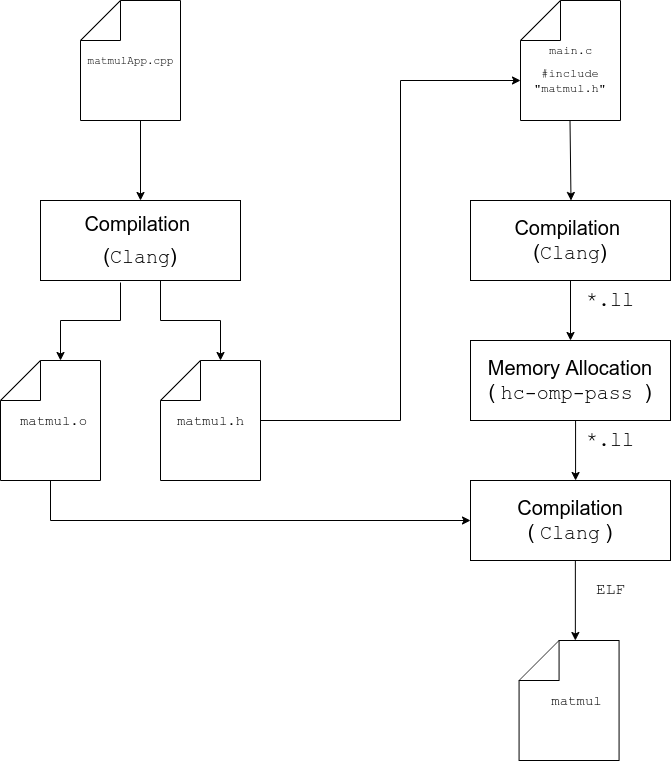
\includegraphics[width=.5\textwidth]{./figures_raw/compilationWorkflow.png}
	\caption{Compilation Workflow for an Halide Application.}
	\label{fig:compwork}
\end{figure}

\begin{figure}[h]
\dirtree{%
	.1 halide-examples/.
	.2 common/.
	.3 defaultHalide.mk.
	.2 myApp/.
	.3 main.c.
	.3 Makefile.
	.3 lib/.
	.4 halidePipeline.cpp.
	}
	\caption{Directory structure for Halide applications.}
	\label{Fig:DirectoryStructure}
\end{figure}


	Figure~\ref{fig:compwork} shows the whole compilation process to build a Halide application for \gls{hero}.
	Every application follows the directory structure described in Figure~\ref{Fig:DirectoryStructure}, the \texttt{common} folder is shared between all the applications and contains a common \texttt{Makefile} that will be included in every application's \texttt{MakeFile}.

	The compilation is done in two steps. First, we compile the Halide pipeline to a RISC-V object file and generate a header file.
	This header file must be included in the hero application (\texttt{main.c}).

	The application building process is based on the \gls{openmp} workflow, we follow the same steps until the final linking phase, more information about the whole process can be found in Koen Wolters's report~\cite{Report:SoftwareStack}.

	We first compile the  source code to \gls{llvm} assembly code. Then due to the heterogeneous nature of the system, a custom program: \texttt{hc-omp-pass} changes every part of the code that may cause issue due to architectural differences between the host and the \gls{pcma} (on \gls{hero}v3, the host is a 64 bits RISC-V processor).
	In our case, as we only compile for the \gls{pulp} cluster, this step does not affect the code, but it will be useful to support the full \gls{hero} platform. 
	Then we use the \gls{llvm} assembly files coupled with the pipeline object file to generate the final binary.


	%%%%%%%%%%%%%
	The header file generated by Halide enumerates every function available on Halide and required to have a fully working Halide implementation. Most of them as not essential and thus do not need to be implemented right away.
	Halide relies on a small subset of functions and we only need to port them for our examples to run. Hopefully, every function or structure in the pipeline header is documented so we can guess which functions are needed.
	We implemented the necessary functions in the \gls{pulp} runtime to make the parallel schedule work, as this is the schedule that will take advantage of the high core count of the cluster.
 
\section{Schedule Implementation }
	Most of the schedules implemented on halide does not require any platform-specific implementation as they are working on the intermediate representation of the source code, but we still have to modify the \gls{pulp} runtime to overload the memory management functions and define the atomic operations which are specific to RISC-V.

    \subsection{Modification to the \acrshort{pulp} runtime}

    The missing halide functions needs to be accessible to the \gls{pulp} runtime, to do so, we created a new file in the kernel (\texttt{halide\_api.c}). 
    This file contains all the basic functions required to run halide on \gls{hero}.

\begin{lstlisting}[language=C,caption={The \texttt{halide\_do\_par\_for} function.},label={lst:halidedoparfor},captionpos=b]
int halide_do_par_for(void *user_context,halide_task_t task,
	int min, int size, uint8_t *closure) {
// Mount the cluster
	rt_cluster_mount(1, 0, 0, NULL);

	unsigned arguments[4];
	arguments[0] = (unsigned)user_context;
	arguments[1] = (unsigned)size;
	arguments[2] = (unsigned)closure;
	arguments[3] = (unsigned)task;

	// Dispatch the task to the cluster
	rt_team_fork(0, pulp_do_halide_par_for_fork, arguments);

	// Unmount the cluster
	rt_cluster_mount(0, 0, 0, NULL);

	return 0;
}
\end{lstlisting}

	The Listing~\ref{lst:halidedoparfor} shows the full source code of the \texttt{halide\_do\_par\_for} function.
	This function is called by halide when a parallel schedule is used. Its role is to distribute on task to the cluster.
	In the first time, \texttt{halide\_do\_par\_for} mount the \gls{pulp} cluster, if the cluster was previously turned off, it is turned back on again.
	The \texttt{argument} structure describe all the informations about the tasks: \texttt{argument[1]} is the total number of task we are going to execute, \texttt{argument[3]} the pipeline function that will be run.
	The core have no way of selecting by themself which task they are going to execute, if we distribute directly the pipeline function, they are all going to execute the same functions with the same arguments.
	To solve this issue we created a wrapper around the pipeline which allow each core to select the tasks based on their core identifier.

	When the execution complete, the cluster is unmounted unsing another \texttt{rt\_cluster\_mount} call.

\begin{lstlisting}[language=C,caption={The \texttt{halide\_do\_par\_for\_fork} function.},label={lst:halidedoparforfork},captionpos=b]
void pulp_do_halide_par_for_fork(void *arg) {
  unsigned *arguments = (unsigned *)arg;

  void *user_context = (void *)arguments[0];
  unsigned task_num = arguments[1];
  uint8_t *closure = (uint8_t *)arguments[2];
  halide_task_t task = (halide_task_t)arguments[3];

  for (unsigned core_id = rt_core_id(); core_id < task_num; core_id += (int)&__rt_nb_pe) {
    task(user_context, core_id, closure);
  }

}
\end{lstlisting}


\iffalse
	%%%%%%%%%%%%%%%%%%%%%%%%%%
	\gls{llvm} does not support yet the \gls{pulp} \gls{simd} extension, but the vectorize schedule may still be used, as Halide will reshape the code as if it was manipulating vectors.
	%%%%%%%%%%%%%%%%%%%%%%%%%%
\fi


 %%% WORK ON THE COMPILATION WORKFLOW



\iffalse
    \subsection{Compiling for the  full platform}
    This process only works on the hardware simulation, and I did not achieved to make it work on the full \gls{hero} platform.
    I tried to approach the question using different strategy. The first one was to use the already compiled object file and add it during the linking process. This method did not work as Clang did not have any indication to distribute the code on the \gls{pulp} cluster. So the RISC-V object file was incompatible.

    The second idea was to use Halide to output C code and include the source in the \gls{hero} application. The issue is that the output of Halide is not pure C code, the pipeline function is coded in C but some structures are still using C++ style. The output needs to be modified by hand to be included in the application. But even after those modifications, the header creates incompatibilities, and thus this method is not usable.

    The last idea was to use the \gls{openmp} \texttt{\#pragma} call to distribute the execution of the function to the \gls{pulp} cluster, and then use the \gls{llvm} assembly file of the pipeline to include it in the application.
    As the first step of the compilation process for \gls{openmp} uses the \gls{llvm} assembly files to compute the offsets in memory, this method may be the best one to compile a Halide application for \gls{hero}.
    But I didn't have enough time to make the heterogeneous compilation work, so this method might not work.
\fi
